\subsubsection{Deep Symbolic Regression for Recurrent Sequences}

\citet{dascoli2022deep} provide the most direct precedent in this review for
sampling a symbolic discrete-time mechanism first and generating a numerical
sequence from it afterward. Their learning task reverses that process: given
the observed initial terms of a sequence, a Transformer predicts a symbolic
recurrence relation capable of generating its continuation. Each synthetic
example is therefore constructed as the paired object

\begin{equation}
    \left(
        \{u_0,u_1,\ldots,u_{n_{\mathrm{input}}-1}\},
        \mathcal{T}
    \right),
    \qquad
    u_n
    =F_{\mathcal{T}}
      \left(n,u_{n-1},\ldots,u_{n-d_{\mathrm{rec}}}\right),
\end{equation}

where $\mathcal{T}$ is both an executable generator and the symbolic target of
the model. Conceptually, the data-generation direction is

\begin{equation}
    \boxed{
    \begin{aligned}
    \text{sample expression tree }\mathcal{T}
    &\;\longrightarrow\; \text{recurrence }F_{\mathcal{T}},\\
    \left(F_{\mathcal{T}},\text{ initial conditions}\right)
    &\;\longrightarrow\; \text{generated sequence}.
    \end{aligned}
    }
\end{equation}

\paragraph{How the recurrence formula is sampled.}
Section~2.1 of \citet{dascoli2022deep} defines the following procedure.

\begin{enumerate}
    \item Sample an operator count $o\in\{1,\ldots,o_{\max}\}$ and construct a
    unary--binary tree with $o$ operator nodes. Larger values of $o$ produce
    syntactically more complex recurrences.

    \item Label every internal node with an operator. In the floating-point
    setting, unary choices are absolute value, square, square root, inverse,
    logarithm, exponential, sine, cosine, tangent, and arctangent; binary
    choices are addition, subtraction, multiplication, and division.

    \item Sample a provisional recurrence degree, then label each leaf as a
    numerical constant, the current index $n$, or a historical term
    $u_{n-i}$ with $1\leq i\leq d_{\mathrm{rec}}$. The three leaf categories
    have equal probability in the reported generator.

    \item Recalculate $d_{\mathrm{rec}}$ from the deepest historical leaf that
    actually occurs in the completed tree, and sample the required initial
    values $u_0,\ldots,u_{d_{\mathrm{rec}}-1}$.

    \item Execute $F_{\mathcal{T}}$ recursively to produce each later term.
    Generation is interrupted when an operator leaves its valid domain or a
    term exceeds the permitted numerical range.
\end{enumerate}

The reported settings are $d_{\max}=6$, $o_{\max}=10$, continuation length
$l\in[5,30]$, equal leaf-category probabilities of $1/3$, and initial values
sampled from $\mathcal{U}(-10,10)$ (paper Table~5). For example, a sampled tree
may encode

\begin{equation}
    u_n=0.7u_{n-1}+\sin(u_{n-3}).
\end{equation}

\begin{figure}[H]
\centering
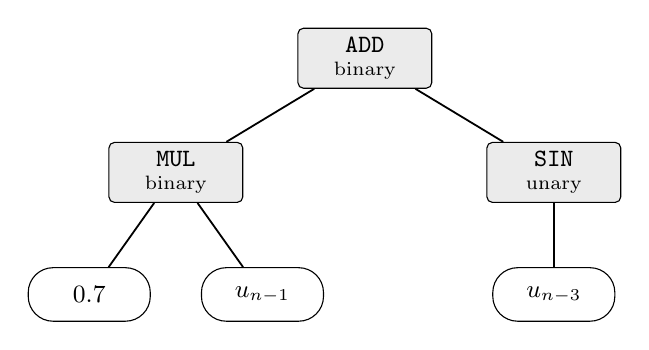
\begin{tikzpicture}[
    operator/.style={
        draw,
        rounded corners=2pt,
        fill=black!8,
        minimum width=1.7cm,
        minimum height=0.72cm,
        align=center,
        font=\small
    },
    leaf/.style={
        draw,
        rounded corners=9pt,
        fill=white,
        minimum width=1.55cm,
        minimum height=0.68cm,
        align=center,
        font=\small
    },
    branch/.style={draw, line width=0.65pt}
]
    \node[operator] (add) at (0,0)
        {\texttt{ADD}\\[-1mm]{\scriptsize binary}};
    \node[operator] (mul) at (-2.4,-1.45)
        {\texttt{MUL}\\[-1mm]{\scriptsize binary}};
    \node[operator] (sin) at (2.4,-1.45)
        {\texttt{SIN}\\[-1mm]{\scriptsize unary}};

    \node[leaf] (constant) at (-3.5,-3.0) {$0.7$};
    \node[leaf] (lagone) at (-1.3,-3.0) {$u_{n-1}$};
    \node[leaf] (lagthree) at (2.4,-3.0) {$u_{n-3}$};

    \draw[branch] (add) -- (mul);
    \draw[branch] (add) -- (sin);
    \draw[branch] (mul) -- (constant);
    \draw[branch] (mul) -- (lagone);
    \draw[branch] (sin) -- (lagthree);
\end{tikzpicture}
\caption{Example unary--binary tree for
$u_n=0.7u_{n-1}+\sin(u_{n-3})$. Binary nodes have two children, the unary
\texttt{SIN} node has one child, and the leaves contain a constant or a lagged
sequence term.}
\label{fig:dascoli-unary-binary-tree}
\end{figure}

Reading Fig.~\ref{fig:dascoli-unary-binary-tree} from the root and recursively
visiting each subtree from left to right produces the prefix representation.
The same tree is serialized in prefix, or Polish, notation, giving a target
such as
\[
    [\texttt{add},\texttt{mul},0.7,u_{n-1},
      \texttt{sin},u_{n-3}].
\]
This representation preserves tree structure without parentheses and allows
the Transformer decoder to generate the recurrence as a token sequence.

\paragraph{How a recovered formula is evaluated.}
Different syntax trees can express the same numerical mechanism. Consequently,
the paper evaluates a predicted recurrence behaviorally: it executes the
predicted and reference formulas from the same initial conditions and checks
the relative error of the next $n_{\mathrm{pred}}$ terms against a tolerance.
This avoids treating an algebraically equivalent expression as wrong merely
because its tokens differ. Beam candidates can likewise be ranked by executing
them and measuring how well they reconstruct the observed sequence.

\paragraph{Contribution to the proposed benchmark.}
This work supplies an expression-first formula sampler for the present thesis:
sample a valid abstract syntax tree, retain that tree as the auditable
mechanism, and execute it to obtain observations. The thesis can extend the
leaf vocabulary with explicit multivariate operators such as
$\operatorname{LAG}(j,\ell)$ and extend the grammar with stochastic
innovations, regime switches, and controlled interaction nodes. Retaining the
sampled tree then supports several references from the same example: its exact
symbolic equation, variable--lag support, signed coefficients when defined,
realized local term values, and generator-based attributions. In the original
study, the tree supervises symbolic-recurrence recovery; in this benchmark, the
same retained mechanism additionally anchors explanation-ground-truth
generation and comparison with forecasting and XAI methods.

